\documentclass[9pt,xcolor=table]{beamer}


\mode<presentation>
{
  \usetheme{metropolis}      % or try Darmstadt, Madrid, Warsaw, ...
  \usecolortheme{seahorse} % or try albatross, beaver, crane, ...
  \usefonttheme{default}  % or try serif, structurebold, ...
  \setbeamertemplate{navigation symbols}{}
  \setbeamertemplate{caption}[numbered]
} 

\makeatletter
\newif\if@mathitemize
\newif\if@closemathitem
\let\orig@item=\item
\renewcommand{\item}{\if@closemathitem$\fi\orig@item\if@mathitemize\@closemathitemtrue$\fi}
\newenvironment{mathitemize}{\@mathitemizetrue\itemize\@closemathitemfalse}{$\enditemize}
\makeatother

\makeatletter
\newcommand{\mtmathitem}{%
\xpatchcmd{\item}{\@inmatherr\item}{\relax\ifmmode$\fi}{}{\errmessage{Patching of \noexpand\item failed}}
\xapptocmd{\@item}{$}{}{\errmessage{appending to \noexpand\@item failed}}}
\makeatother

\newenvironment{mathitem}[1][]{%
\itemize[#1]\mtmathitem}{$\endlist}                    %$

\newenvironment{mathenum}[1][]{%
\enumerate[#1]\mtmathitem}{$\endlist}                  %$

\newenvironment{mathdesc}[1][]{%
\description[#1]\mtmathitem}{$\endlist} 

\usepackage{ragged2e}
\usepackage{etoolbox}
\usepackage{lipsum}
\usepackage[absolute,overlay]{textpos}
\usepackage{graphicx}
\usepackage{rotating}
\usepackage{multirow}
\usepackage{changepage}

\apptocmd{\frame}{}{\justifying}{}

\usepackage[english]{babel}
%\usepackage[utf8x]{inputenc}
\usepackage{colortbl}
\graphicspath {{figures/}}
\usepackage[font=scriptsize,labelfont=bf]{caption}


\setbeamercolor{bibliography item}{parent=palette primary}
\setbeamertemplate{bibliography entry title}{}
\setbeamertemplate{bibliography entry location}{}
\setbeamertemplate{bibliography entry note}{}
\setbeamertemplate{bibliography item}{\insertbiblabel}


%% GRID %%
\usepackage{tikz}
\usetikzlibrary{arrows,decorations.markings}
\usetikzlibrary{decorations.pathreplacing}

\newcommand{\grid}{
 \begin{tikzpicture}[overlay,remember picture]
   \begin{scope}[shift={(current page.south west)}]
     \draw[gray!50] (0,0) grid[step=2mm] (current page.north east);
     \draw[red!50] (0,0) grid[step=1cm] (current page.north east);
     \draw (0.2,1) node {1};
     \draw (0.2,2) node {2};
     \draw (0.2,3) node {3};
     \draw (0.2,4) node {4};
     \draw (0.2,5) node {5};
     \draw (0.2,6) node {6};
     \draw (0.2,7) node {7};
     \draw (0.2,8) node {8};
     \draw (0.2,9) node {9};
     \draw (1,0.5) node {1};
     \draw (2,0.5) node {2};
     \draw (3,0.5) node {3};
     \draw (4,0.5) node {4};
     \draw (5,0.5) node {5};
     \draw (6,0.5) node {6};
     \draw (7,0.5) node {7};
     \draw (8,0.5) node {8};
     \draw (9,0.5) node {9};
     \draw (10,0.5) node {10};
     \draw (11,0.5) node {11};
     \draw (12,0.5) node {12};
   \end{scope}
 \end{tikzpicture}
 }
 
%%

\title{DAIT Project}
\subtitle{Trajectory Preduiction for Human-Human Interaction}
\author{Rodolphe Farrando, Romain Gratier}%\\[1cm] {\small Supervisors: Nicholas Molyneaux, Ga�l Lederrey, Michel Bierlaire}}
\institute{EPFL}
\date{23.05.2018}


\begin{document}

\begin{frame}[noframenumbering]
  \maketitle
  \thispagestyle{empty}
\end{frame}

\begin{frame}[noframenumbering]{Table of contents}
\thispagestyle{empty}
  \setbeamertemplate{section in toc}[sections numbered]
  \vspace{0.6cm}
  \tableofcontents[hideallsubsections]
\end{frame}

%%%%%%%%%%%%%%%%%%%%%%% INTRODUCTION %%%%%%%%%%%%%%%%%%%%%%% 

\section{Introduction}
\begin{frame}{Introduction}
\begin{itemize}
\onslide<1->{\item Trajectory prediction is crucial for improving autonomous vehicles behaviour}
\onslide<2->{\item Could avoid situations seen in the ethical lectures}
\end{itemize}

\begin{center}
\begin{overprint}
\onslide<1> \centerline {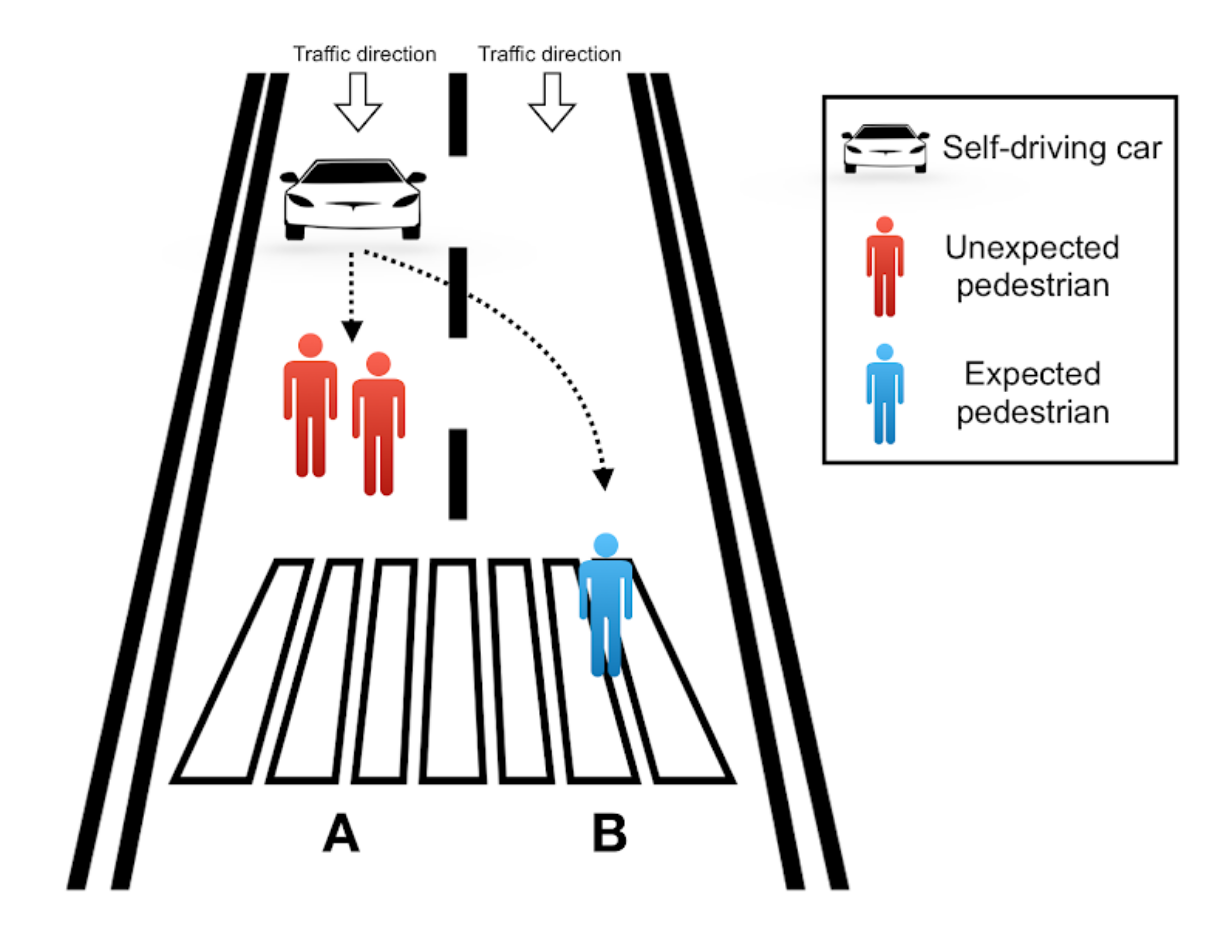
\includegraphics[scale = 0.32]{figure/intro1}}
\onslide<2->\centerline {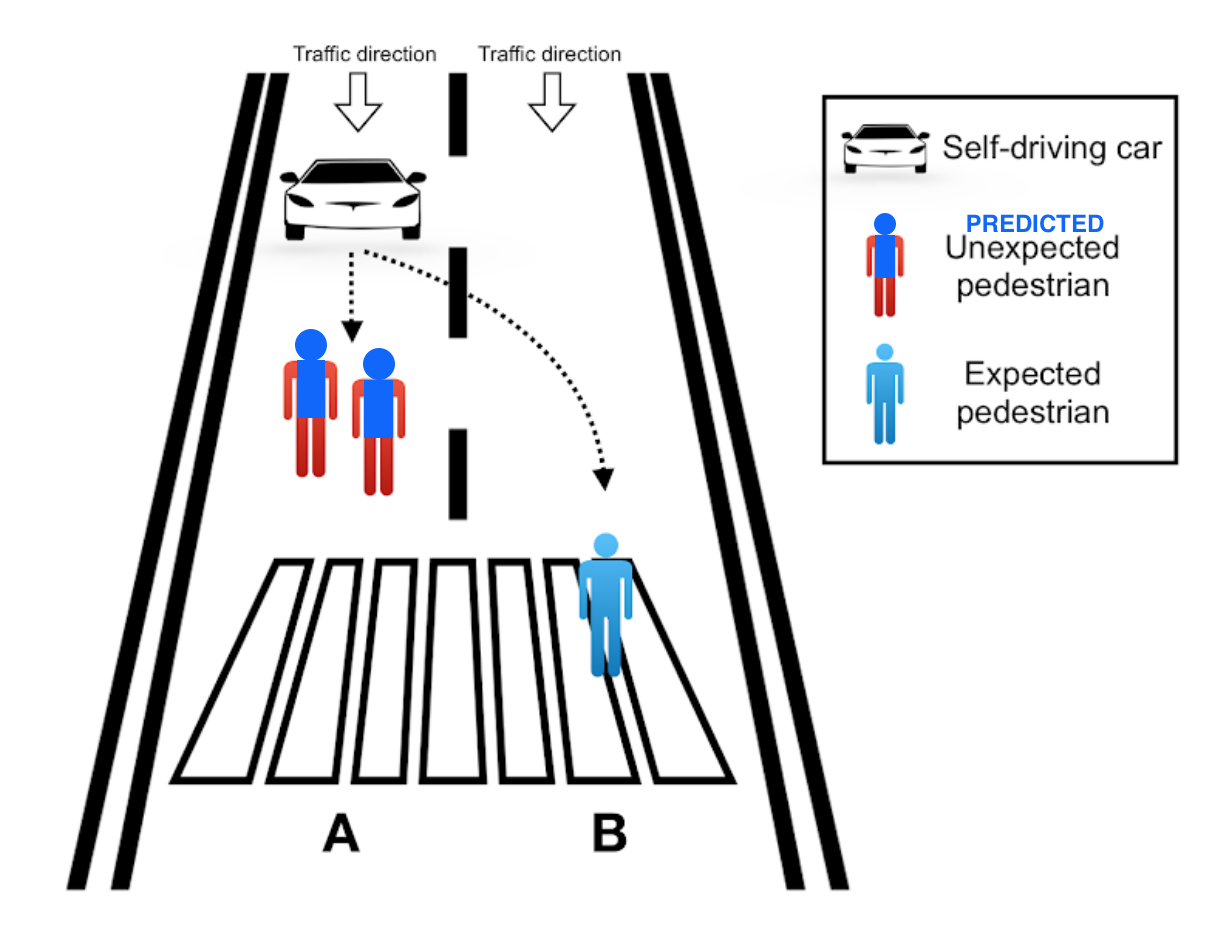
\includegraphics[scale = 0.32]{figure/intro2}}
\end{overprint}
\end{center}


%Goal:
%\begin{itemize}
%\item Find model which predict trajectories better than linear prediction
%\item Predict coordinates
%\end{itemize}
\end{frame}
%%%%%%%%%%%%%%%%%%%%%%% LITERATURE %%%%%%%%%%%%%%%%%%%%%%% 

\begin{frame}{Previous work Social LSTM : Human Trajectory Prediction in Crowded Spaces}
%\begin{block}{Social LSTM : Human Trajectory Prediction in Crowded Spaces}
%\end{block}

\begin{columns}[T] % align columns
\begin{column}{.48\textwidth}
In their project, they used different components to make the structure:\\
\begin{itemize}
\item One LSTM per pedestrian
\item Social Pooling
\item Prediction per frame
\end{itemize}
\vspace{1.2cm}
\onslide<2->{In our project we only use:\\
\begin{itemize}
\item One CNN, or one LSTM
\item Prediction per pedestrian
\end{itemize}}
\end{column}%

\hfill%


\begin{column}{.48\textwidth}
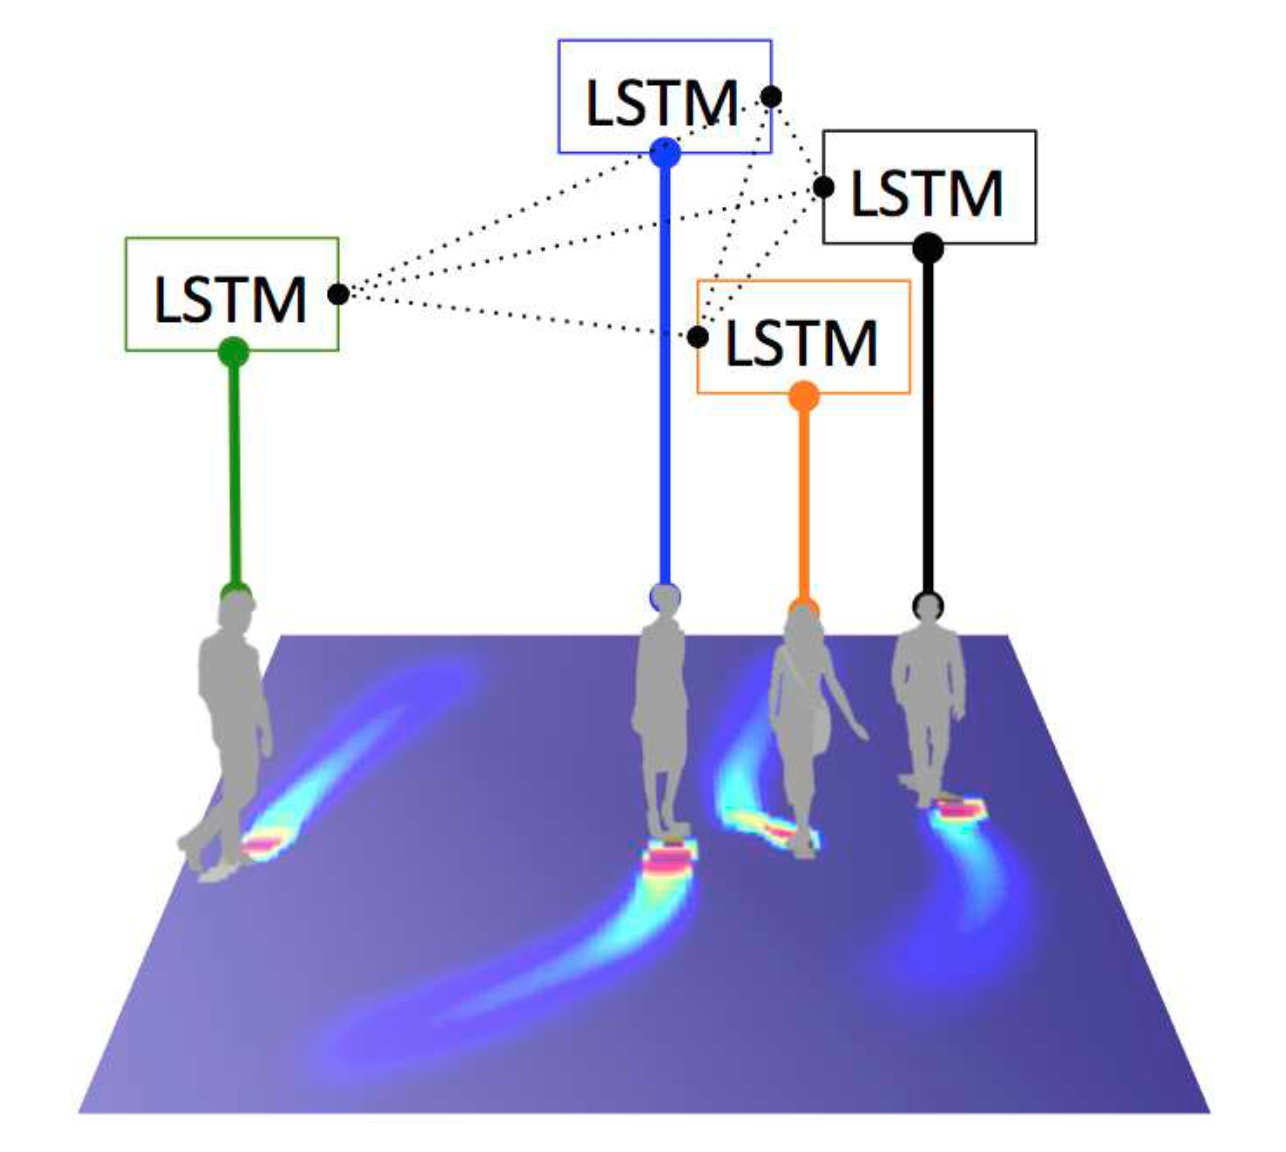
\includegraphics[scale = 0.17]{figure/socialLSTM}
\vspace{0.2cm}
\onslide<2->{\includegraphics[scale = 0.23]{figure/OurModel}}
\end{column}%
\end{columns}
\vspace{0.2cm}
\tiny{\emph{Images from Social LSTM:Human Trajectory Prediction in Crowded Spaces and courses lecture}}
\end{frame}


%%%%%%%%%%%%%%%%%%%% PREPROCESSING %%%%%%%%%%%%%%%
\section{Data}




\begin{frame}{Pre-processing}
The preprocessing is divided in 4 steps:
\begin{enumerate}
\justifying
\onslide<1->{\item We isolate each trajectory along with his interaction, that is the other trajectories that are around within the same frames}
\onslide<2->{\item We normalize the trajectories such that the first point is at $(0,0)$ and the second is at $(0,y_1)$}
\onslide<3->{\item We calculate axis velocities $V_x$ and $V_y$}
\onslide<4->{\item For each frame, if there is a interacting pedestrian we add its coordinates and speed otherwise zeros are added}
\onslide<5->{\item Data augmentation (flip and add noise) cf. last slide}
\end{enumerate}
\begin{center}
\begin{overprint}
\onslide<1> \centerline {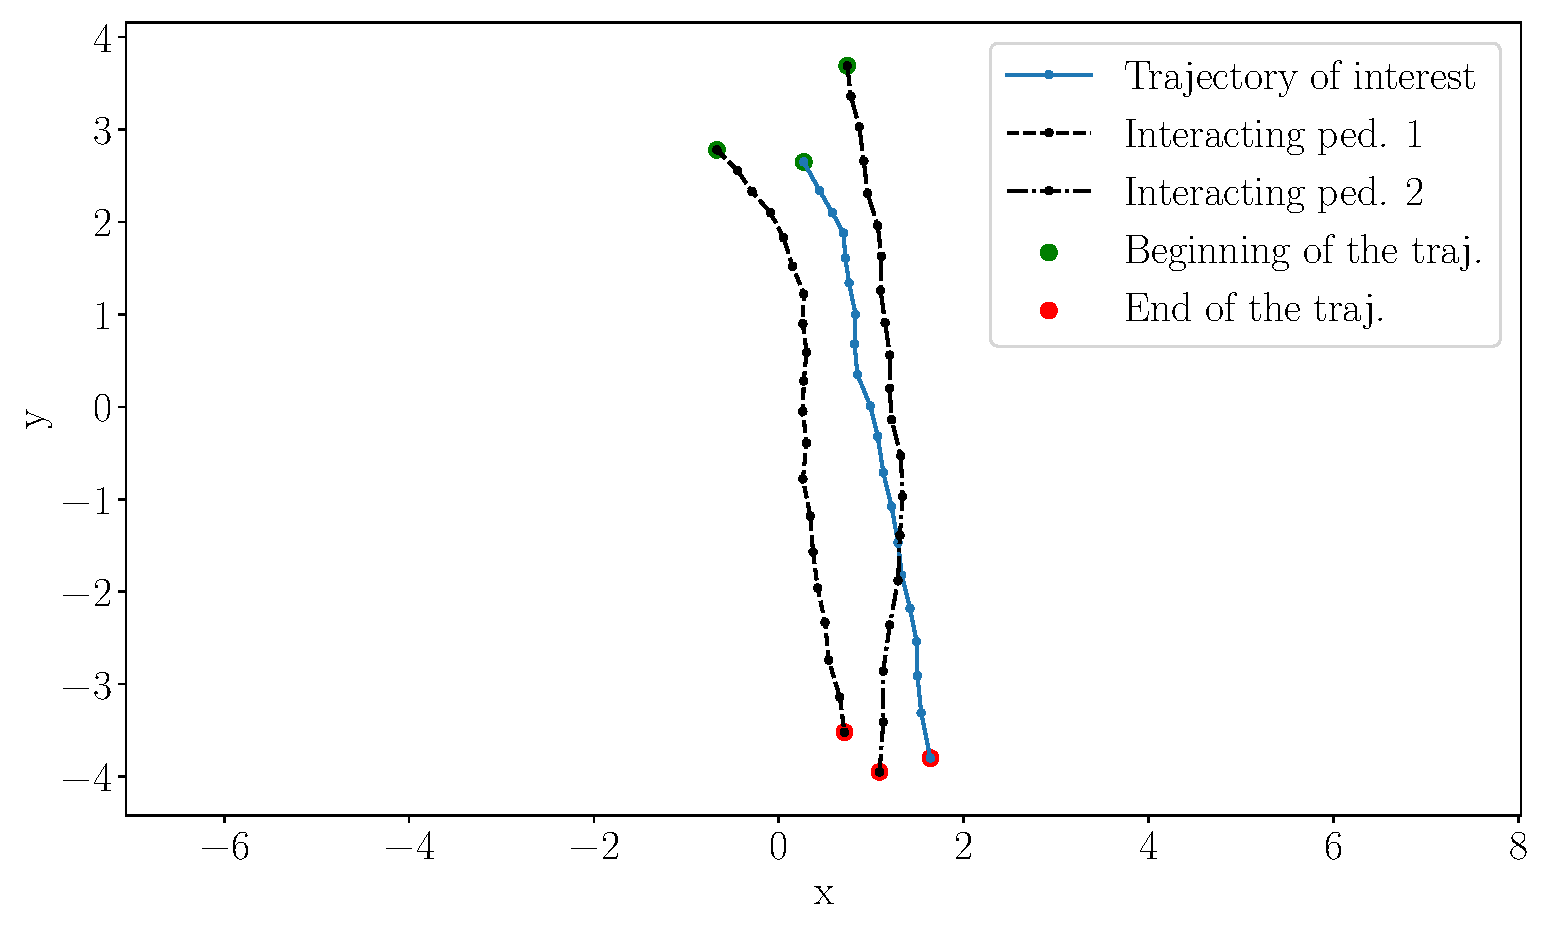
\includegraphics[scale = 0.25]{figure/beforerot}}
\onslide<2->\centerline {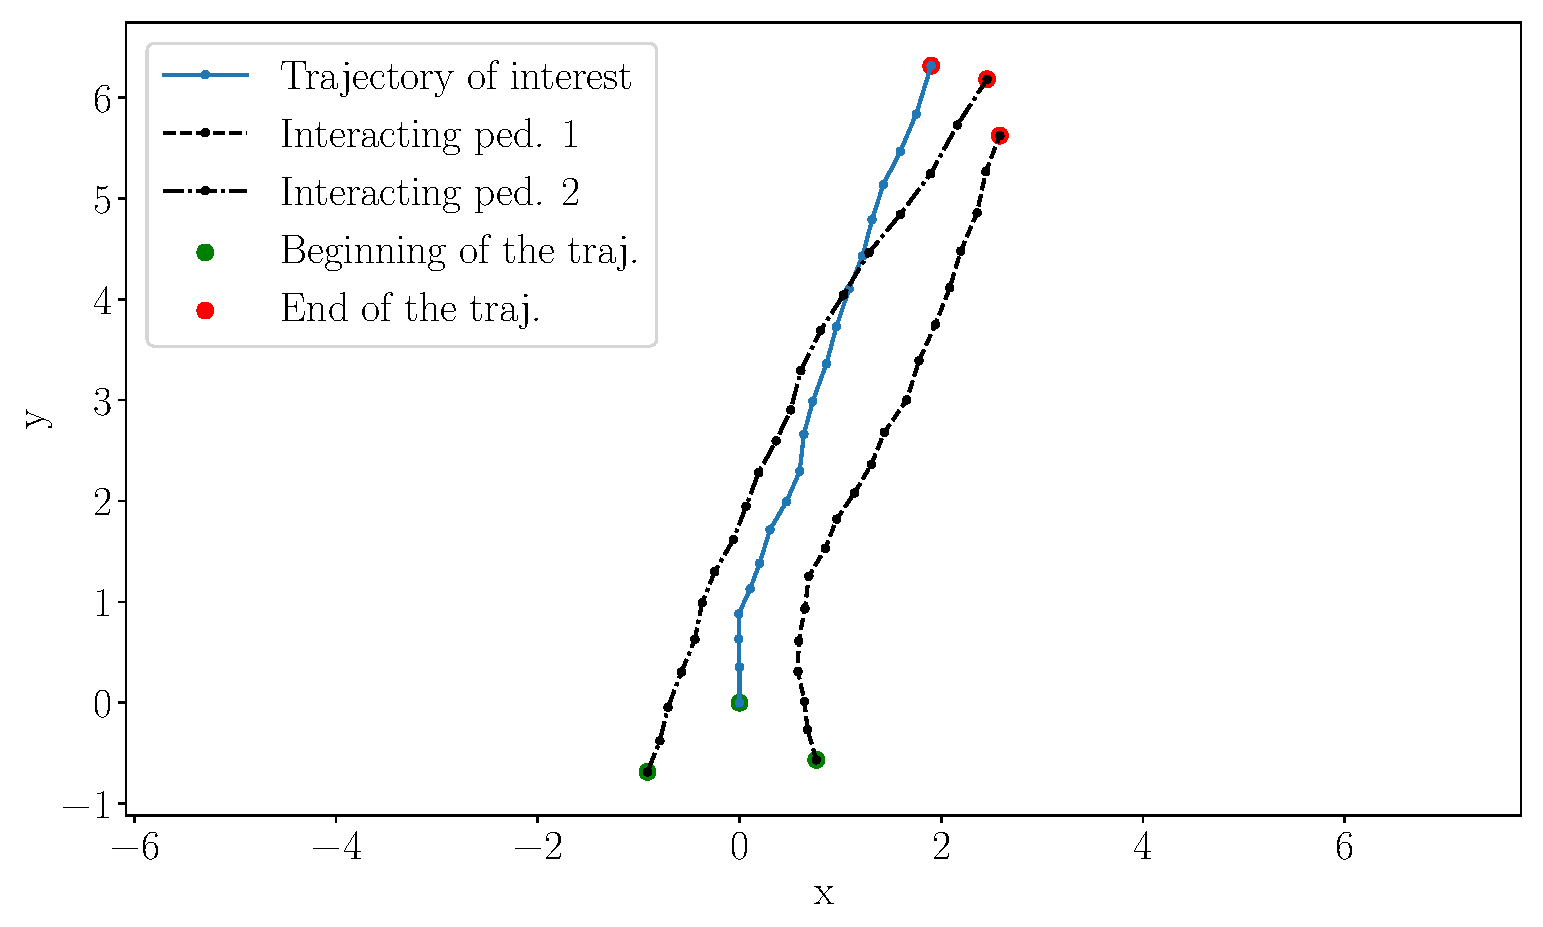
\includegraphics[scale = 0.25]{figure/afterrot}}
\end{overprint}
\end{center}
\end{frame}

\begin{frame}{Data}

\begin{columns}[T] % align columns
\begin{column}{.38\textwidth}
We have a file with:
\begin{itemize}
\justifying
\item Pedestrians ID
\item Frame number 
\item Twenty sets of $x$ and $y$ coordinates per pedestrian
\end{itemize}
\vspace{0.5cm}
\onslide<2->{We want :\\
\begin{itemize}
\justifying

\item Train on the 10 first coordinates
\item Predict the next 10 
\end{itemize}}

\end{column}%

\hfill%

% align columns
\begin{column}{.61\textwidth}
\begin{table}[]
\centering
\begin{tabular}{|c|c|c|c|c|c|}
\hline
Frame Number & ID & $x$ & $y$ & $ V_x$ & $V_y$ \\ \hline
        \vdots     &  \vdots  &  \vdots &  \vdots &  \vdots &  \vdots \\ \hline
\end{tabular}
\end{table}
\vspace{0.6cm}
\onslide<2->{
Example of trajectory to predict
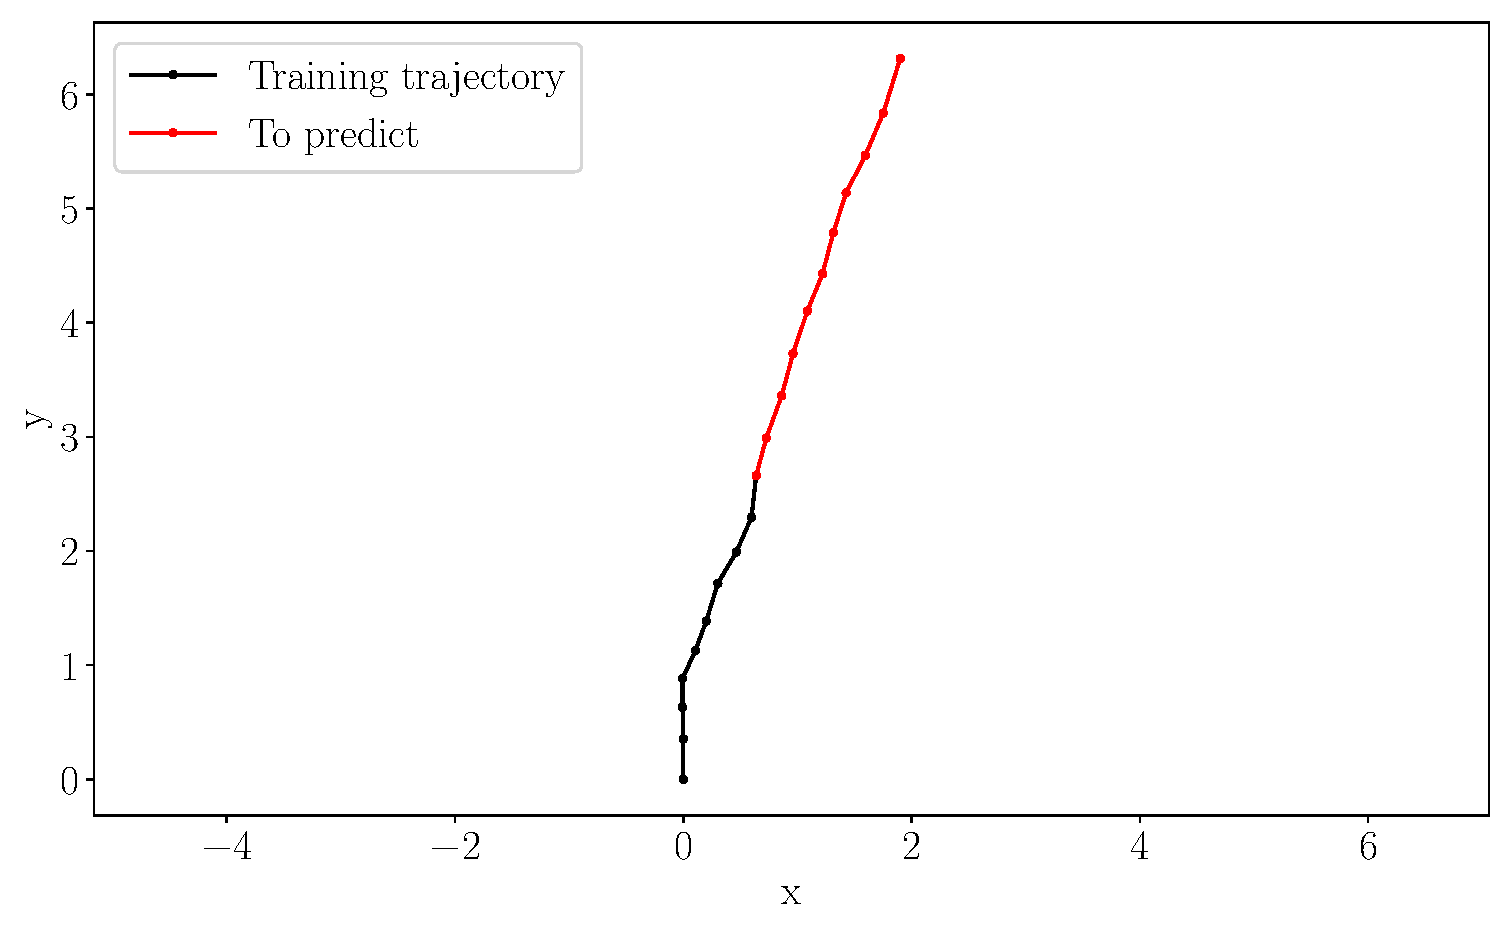
\includegraphics[scale=0.25]{figure/examplepres}
}
\end{column}%
\end{columns}

\end{frame}

\begin{frame}
\frametitle{Outputs structure}
Finally our inputs have the following shape: $[10,N,4 * N_{inter}]$, with 
\begin{itemize}
\justifying
\item 10: sequence length
\item $N$: The number of data
\item $4*N_{inter}$: 4 (being the $x$ and $y$ coordinates and $V_x$ and $V_y$ velocities) times the number of pedestrians interacting with the one of interest.
\end{itemize}
%\begin{itemize}
%\item The models can predict either coordinate or speed or both
%\item We test our two models for 4 different cases
%\end{itemize}
The four different cases are:
\begin{enumerate}
\justifying
\item Predict coordinates with loss defines as $L_1 = (X-X_{pred})^2$ with $X = [x,y]$
\item Predict speeds with loss defines as $L_2 = (V-V_{pred})^2$ with $V = [V_x,V_y]$ 
\item Predict both coordinates and speeds with loss defines as $L = L_1 + L_2$
\item Predict both coordinates and speeds with loss defines as $L = L_1 + L_2 + L_3 $, with $L_3 = (X- X_{t-1} + V_t*0.4)^2$
\end{enumerate}
The fourth case ensure that coordinates and speeds are not predicted independently.
\end{frame}




\section{Models}
\begin{frame}{CNN}
\begin{figure}
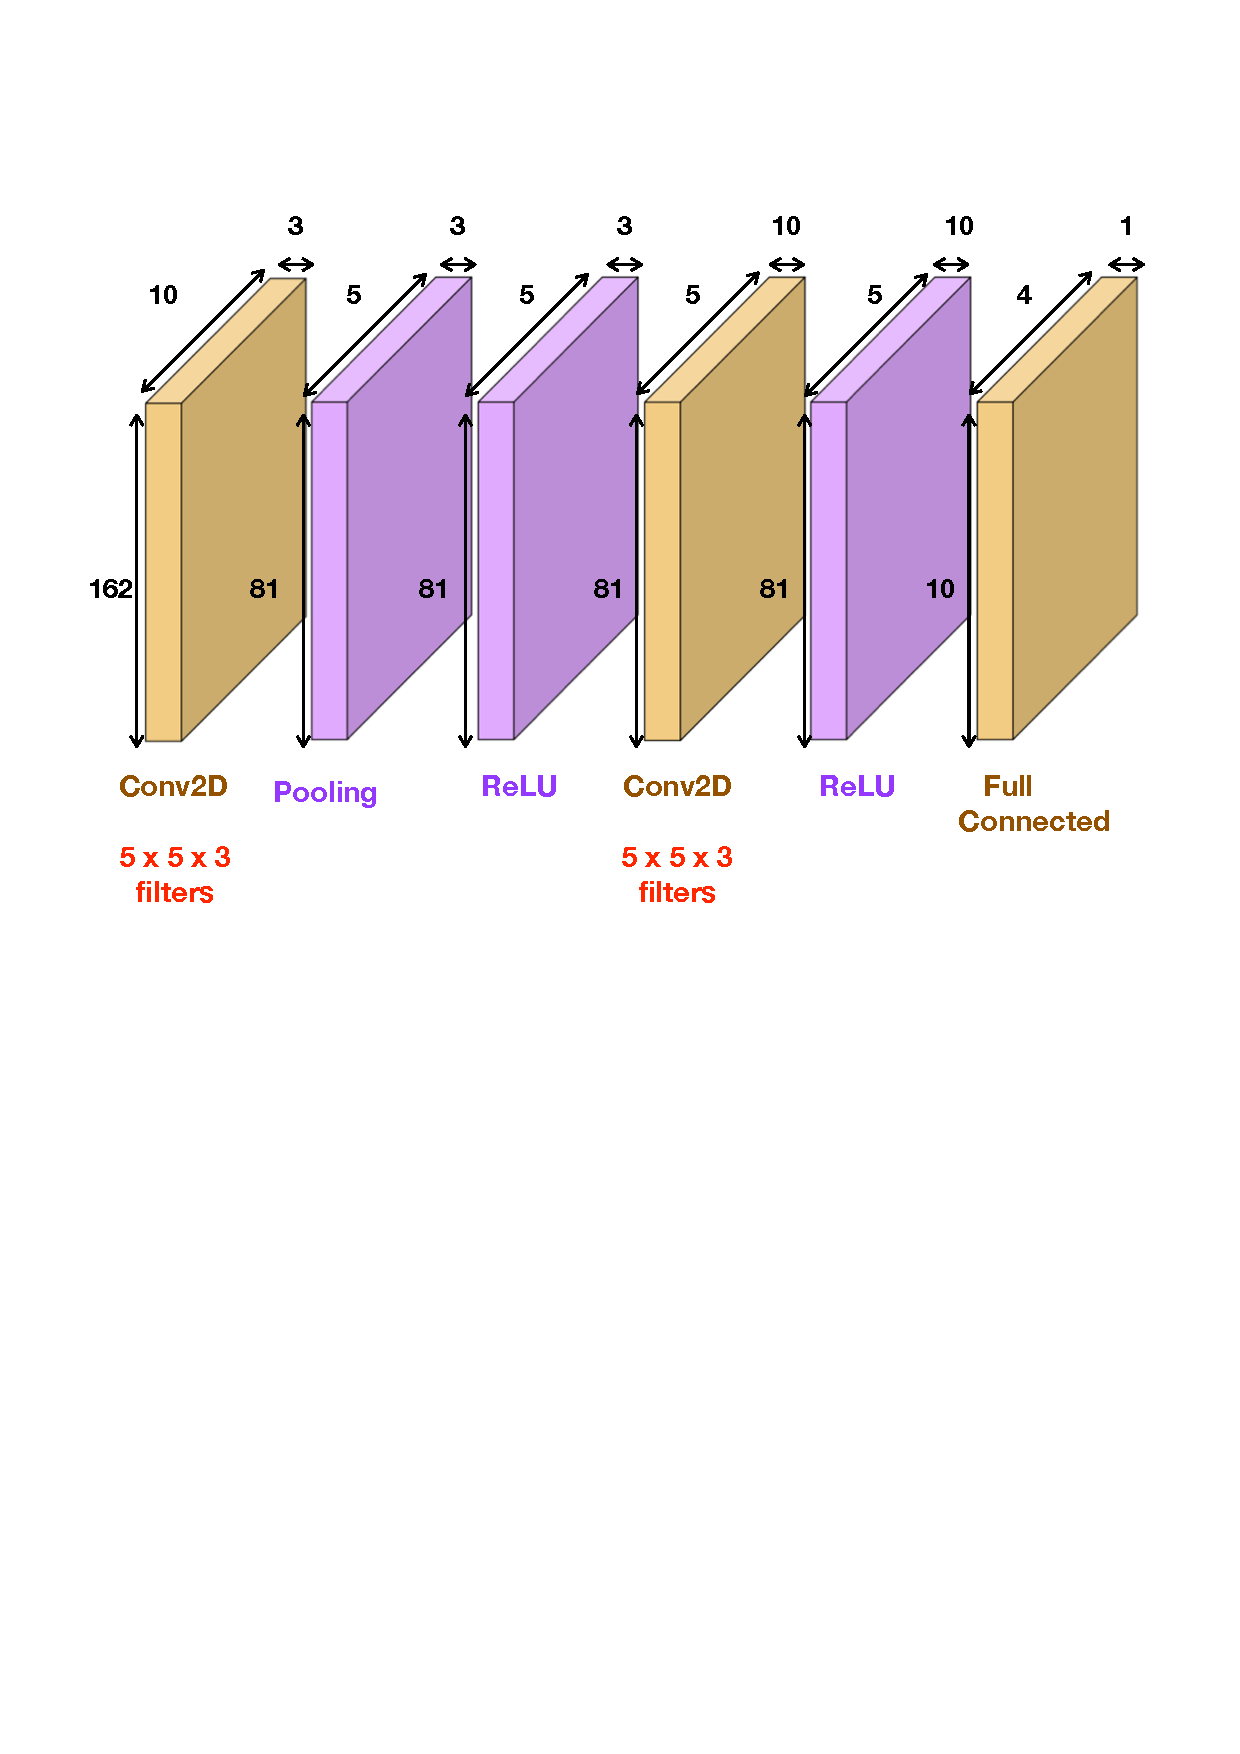
\includegraphics[scale = 0.35]{figure/CNN}
\end{figure}
\textbf{Inputs:} sequence of coordinates and velocities of the pedestrians\\
\textbf{Outputs:} sequence of predicted coordinates and velocities for a trajectory of interest 
\end{frame}

\begin{frame}{LSTM}
\begin{figure}
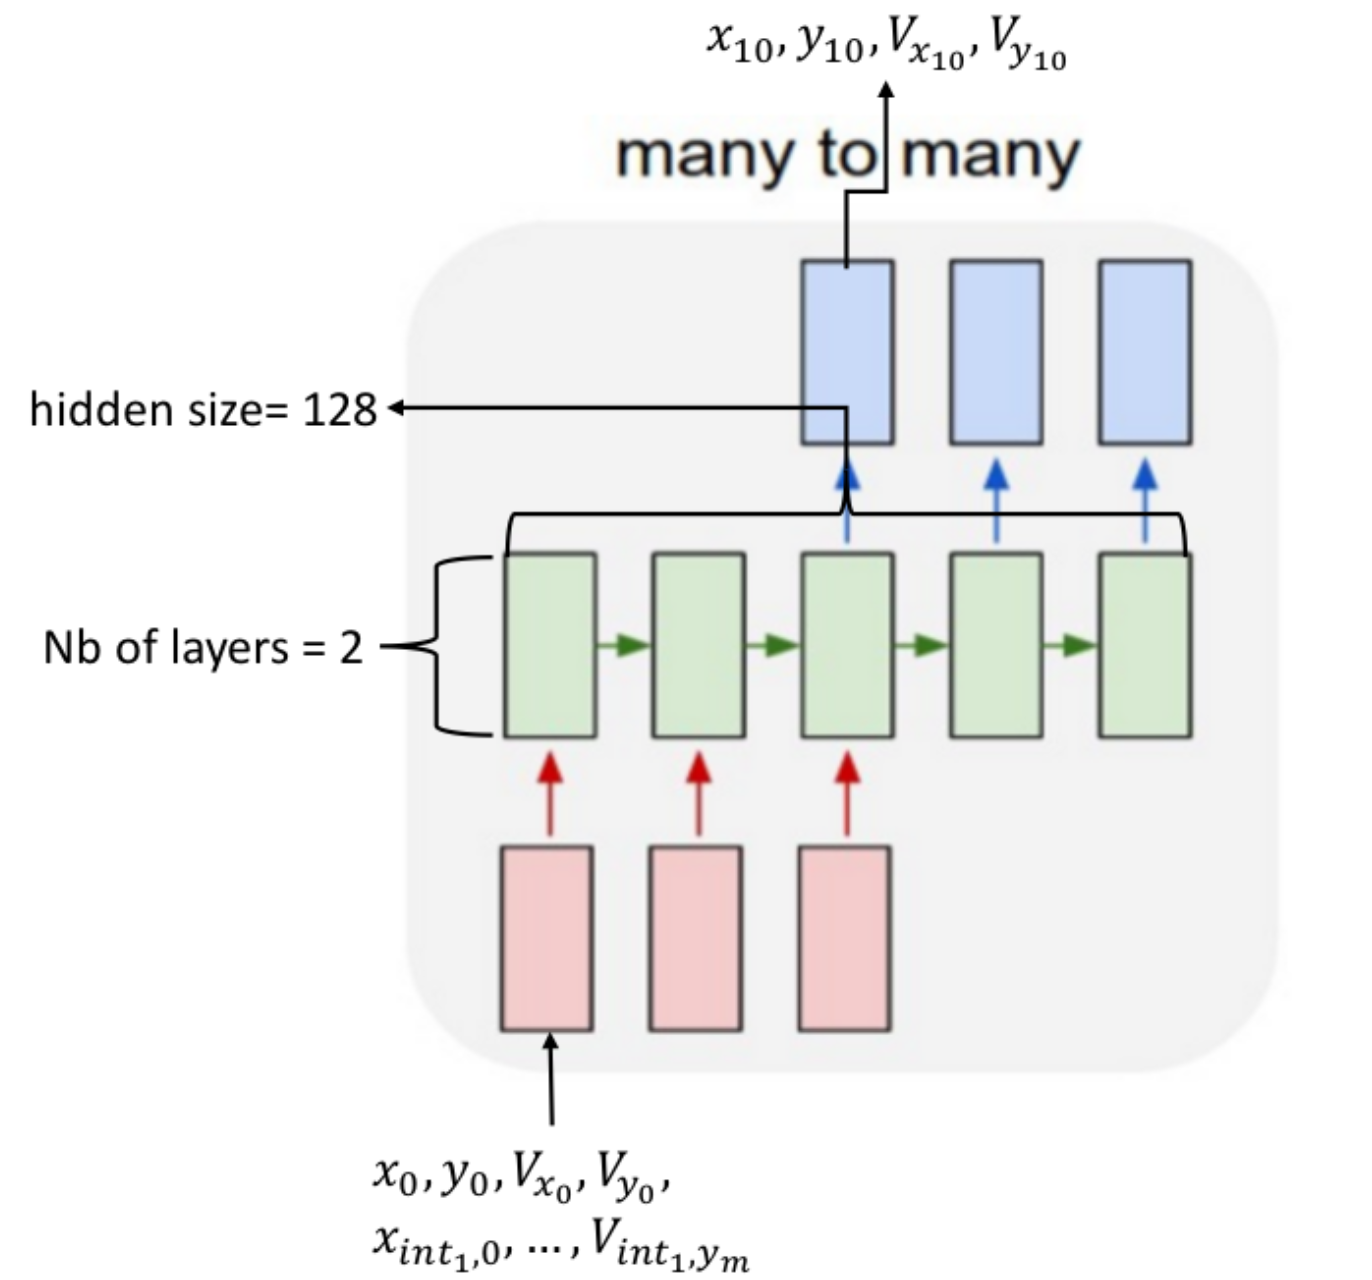
\includegraphics[scale = 0.25]{figure/manytomany}
\end{figure}
\textbf{Inputs:} sequence of coordinates and velocities of the trajectory of interest and of the interacting trajectories\\
\textbf{Outputs:} sequence of predicted coordinates and velocities for the trajectory of interest 
\end{frame}

\section{Results}
\begin{frame}
\frametitle{Results: Introduction}
To calculate the correctness of the prediction two indicators are used:
\begin{enumerate}
\item The final displacement error: $e_{fin} = \sqrt{(X_{n}-X_{pred,n})^2}$
\item The mean displacement error: $e_{fin} = \sqrt{\frac{\sum_{i=0}^n(X_{gt,i}-X_{pred,i})^2}{(n)}}$
\end{enumerate}
Depending on the inputs two ways are possible to find the predicted coordinates:
\begin{enumerate}
\item If the coordinates are predicted: directly use them
\item If the velocities are predicted: $X_{t} = X_{t-1} + V_{t}\cdot 0.4$, with $0.4$ the time between two frames in seconds
\end{enumerate}
Results for both models: 
\begin{itemize}
\item 3 Types of trajectory defined: Static, linear and non-linear trajectories
\item Mean and Final displacements
\end{itemize}

\end{frame}




\begin{frame}
\frametitle{Results}
Linear prediction results:
\begin{itemize}
\item Type 1: \emph{Mean} = 0.141, \emph{Final} = 0.322
\item Type 2: \emph{Mean} = 0.541, \emph{Final} = 0.93
\item Type 3: \emph{Mean} = 0.651, \emph{Final} = 1.457
\item Total: \emph{Mean} = 0.512, \emph{Final} = 0.982 

\end{itemize}
\fontsize{7pt}{8.2}\selectfont
\begin{table}[]
\centering
\begin{adjustwidth}{-2em}{-2em}
\begin{tabular}{cc|c|c|c|c|c|c|c|c|}
\cline{3-10}
\multicolumn{1}{l}{}                                     &                & \multicolumn{4}{c|}{\textbf{CNN}}                                    & \multicolumn{4}{c|}{\textbf{LSTM}}                                                          \\ \cline{3-10} 
                                                         &                & \textbf{Type 1} & \textbf{Type 2} & \textbf{Type 3} & \textbf{Total} & \textbf{Type 1} & \textbf{Type 2} & \textbf{Type 3} & \textbf{Total}                        \\ \hline
\multicolumn{1}{|c|}{}                                   & \textbf{Mean}  &4.696                 & 5.144                &4.674                 &4.176                & 1.16            & 0.768           & 0.817           & 0.837                                 \\ \cline{2-10} 
\multicolumn{1}{|c|}{\multirow{-2}{*}{\textbf{Coord.}}} & \textbf{Final} &10.246                 & 7.009                &10.501                 &5.602                & 1.269           & 0.911           & 1.087           & 1.011                                 \\ \hline
\multicolumn{1}{|c|}{}                                   & \textbf{Mean}  &0.567                 &5.133                 &1.911                 &4.17                & 0.742           & 0.397           & 0.448           & {\color[HTML]{FE0000} \textbf{0.461}} \\ \cline{2-10} 
\multicolumn{1}{|c|}{\multirow{-2}{*}{\textbf{Speed}}} & \textbf{Final} &0.77                 &6.971                 &3.882                 &5.587                & 1.433           & 0.716           & 0.874           & {\color[HTML]{FE0000} \textbf{0.863}} \\ \hline
\multicolumn{1}{|c|}{}                                   & \textbf{Mean}  &1.269       3          &5.134                 &1.762                 &{\color[HTML]{FE0000} \textbf{4.163}}                & 0.519           & 0.484           & 0.568           & 0.511                                 \\ \cline{2-10} 
\multicolumn{1}{|c|}{\multirow{-2}{*}{\textbf{2 Loss}}} & \textbf{Final} &2.727                 &6.978                 &3.546                 &{\color[HTML]{FE0000} \textbf{5.57}}                & 0.979           & 0.871           & 1.093           & 0.946                                 \\ \hline
\multicolumn{1}{|c|}{}                                   & \textbf{Mean}  &0.549                 &5.135                 &3.829                 &4.163                & 0.537           & 0.473           & 0.576           & 0.51                                  \\ \cline{2-10} 
\multicolumn{1}{|c|}{\multirow{-2}{*}{\textbf{3 Loss}}} & \textbf{Final} &0.758                 &6.983                 &4.962                 &5.573                & 0.992           & 0.86            & 1.125           & 0.95                                  \\ \hline
\end{tabular}
\end{adjustwidth}
\end{table}
\end{frame}

\begin{frame}
\frametitle{Results}
Discussion
\end{frame}
\section{Representation}

\begin{frame}
\frametitle{Representation}

\end{frame}

\begin{frame}
\frametitle{Dynamic Representation}

\end{frame}

\begin{frame}
\frametitle{Discussion}


\end{frame}


\end{document}